\section{Travelling Wave Analysis}

%%%%%%%%%%%%%%%%%%%%%%%%%%%%%%%%%%%%%%%%%%%%%%%%%%%%%%%%%%%
\subsection{Spatial Simplification}

To simplify the travelling wave analysis we reduce the spatial dimensions to that of a one dimensional problem.
This can be done if initial conditions that are homogenous with respect to $y$ are chosen.
The purpose of this spatial simplification is that this will speed up the computations considerable.
It will also make visualizations easier as certain figures would become too cluttered in two dimensions.
What is done here is more of a pseudo-reduction of dimensions.
%!% is it n or (n+1) same for m...
By reducing the grids from an $n \times m$ grid to an $n \times 4$ grid we have changed the way the problem size scales with finer grids.
The problem is still two dimensional, just now one dimension has been reduced to only 4 grid points of accuracy instead of $m$ points.
This does not effect the final result since we only apply this change to problems with appropriate initial conditions.
These initial conditions are homogenous in the $y$ direction and thus we do not have any fluctuation between $y$ values for a given $x$ value.

%!% Is it n or (n+1), same for m
One main benefit of changing the grid from $n \times m$ to $n \times 4$ is that the growth of the problem with respect to the resolution of the grid is reduced dramatically.
This changes the problem from a $O(n^2)$ problem to a $O(n)$.
Using the one dimensional travelling wave initial conditions, (\ref{equ:basic_init_trav_wave}), one simulation is computed with a $513 \times 513$ grid, seen at Figure \ref{fig:show_dimension_3D}, and another with a $513 \times 4$ grid, seen at Figure \ref{fig:show_dimension_2D}.

\begin{figure}[!htp]
  \centering
  \begin{tabular}{c c}
    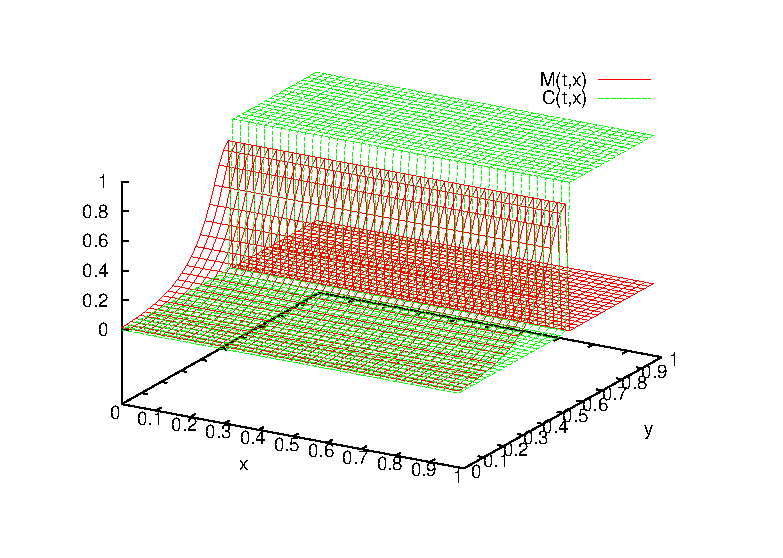
\includegraphics[scale=0.7]{show_dimension_3D.eps} &
    %!% Fix the y axis tics so they don't hidously overlap
    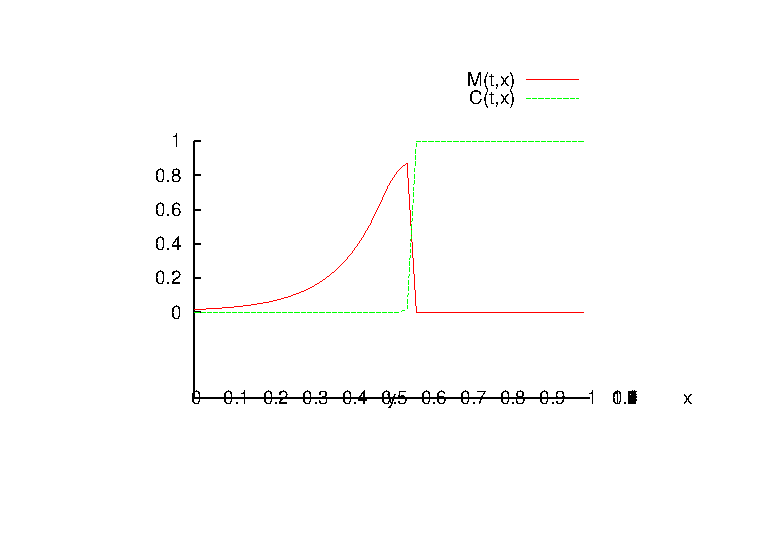
\includegraphics[scale=0.7]{show_dimension_3D_side.eps} \\
    (a) & (b) \\
  \end{tabular}
  \caption{Graph of (a) 3D view of $M(t,x,y)$ and $C(t,x,y)$, (b) Side profile view of $M(t,x,y)$ and $C(t,x,y)$ at $t=40$.} 
  \label{fig:show_dimension_3D}
\end{figure}
   
Before any changes to the grid can be made, it must be confirmed that fluctuations are sufficiently small.
To this end, the standard deviation is used as a measure.
The standard deviation is calculated along the $y$-direction for each x value.
This gives a numerical quantity for the measure of dispersal each $y$ value has with another.
Here, we use the sample standard deviation for the sole reason that this single simulation does not represent its own population.
Initially, at $t =0$ the standard deviation is 0 everywhere (DATA NOT SHOWN).
At $t = 40$, Figure \ref{fig:show_dimension_stddev} show the standard deviation of each $y$ value.
After many time steps have passed the amount of spread is always less then $10^{-14}$, which is an acceptable degree of consistency.
Note that the main inconsistency is at the wave front, around $x = 5.75$, which is mainly because of the sharp change in values.

\begin{figure}[!htp]
  \centering
  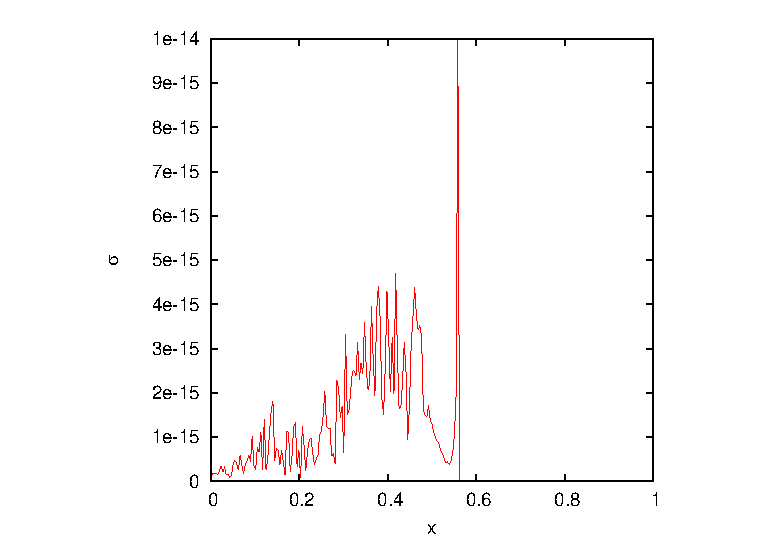
\includegraphics{show_dimension_stddev.eps}
  \caption{The standard deviation at the same time as the above graphs}
  \label{fig:show_dimension_stddev}
\end{figure}

%!% Is it n or n+1?
When simulations are computed with a $n \times 4$ grid, a two dimensional solution is still computed. 
With regards to visualizations, side profiles could be used on these solutions to present pseudo-one dimensional visualizations; this is not ideal.
To visualize the solutions in true one dimension we use $\bar{M}$ and $\bar{C}$ as averaged values of the solutions along the y-axis.
This is computed after the solution has been determined and is independent of the actual computations for M and C.
So by taking the average of the points along the $y$-axis we can get a two dimensional plot as seen in Figure \ref{fig:show_dimension_2D}. 
 
\begin{figure}[!htp]
  \centering
    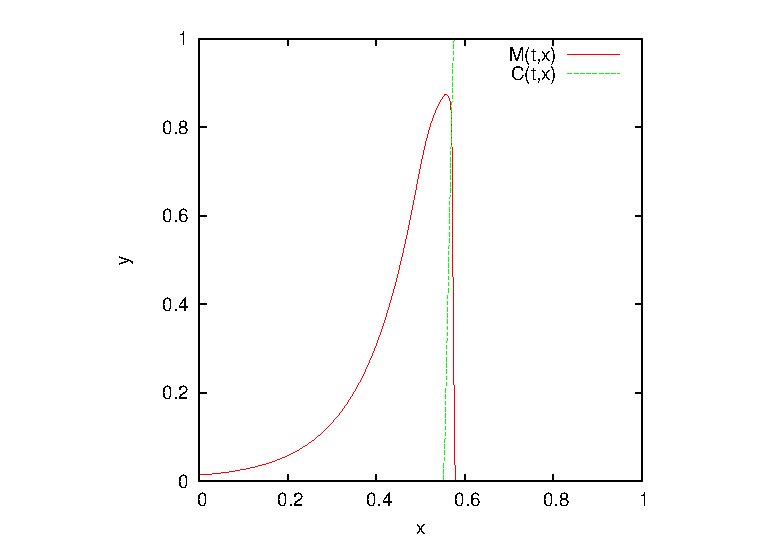
\includegraphics{show_dimension_2D.eps}
    \caption{Graph of M(2,y) and C(2,y), now reduced to a one dimensional solution.}
    \label{fig:show_dimension_2D}
\end{figure}

This means that the system (\ref{equ:model_system}) - (\ref{equ:model_functions}) can be reduced to a one dimensional problem. 
With initial conditions that are homogenous with respect to y, we can greatly reduce the required number of grid points in the one axis.
Once the y-axis reduced, we can also ignore it for visualizations, only using the x-z axis and plotting the values of $\bar{M}$ and $\bar{C}$.


%%%%%%%%%%%%%%%%%%%%%%%%%%%%%%%%%%%%%%%%%%%%%%%%%%%%%%%
\subsection{Travelling Wave Solution}


%!% section 1.2.2 i think before you discuss travelling waves, you should define what they are. Just take it from my old paper
Classical travelling wave solutions are solutions that propagate with an \textit{a priori} unknown constant speed without any change in shape.
This means that the solutions can be defined as 
\begin{equation}
  %!% why \tilde??
  M(t,x) = M(x - ct)
\end{equation}
Figure \ref{fig:trav_wave_solution} shows the time evolution of the single time snapshot from Figure \ref{fig:show_dimension_2D}.
Given the above definition and by looking at the consistent appearance of the solution, it suggests that it is a travelling wave.
It is clear here that the shape of the solution is consistent enough to suggest the existence of a travelling wave solution.

\begin{figure}[!htp]
  \centering
  \begin{tabular}{c c}
      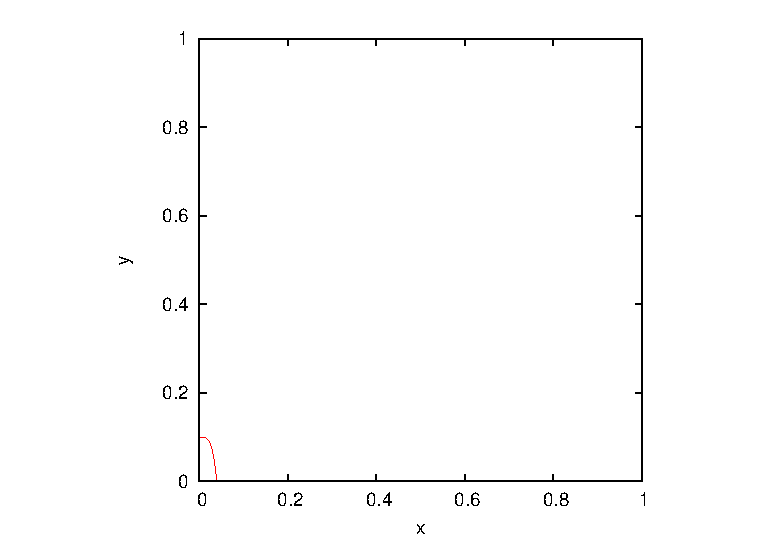
\includegraphics[scale=0.55]{trav_wave_solution_t0.eps} &
      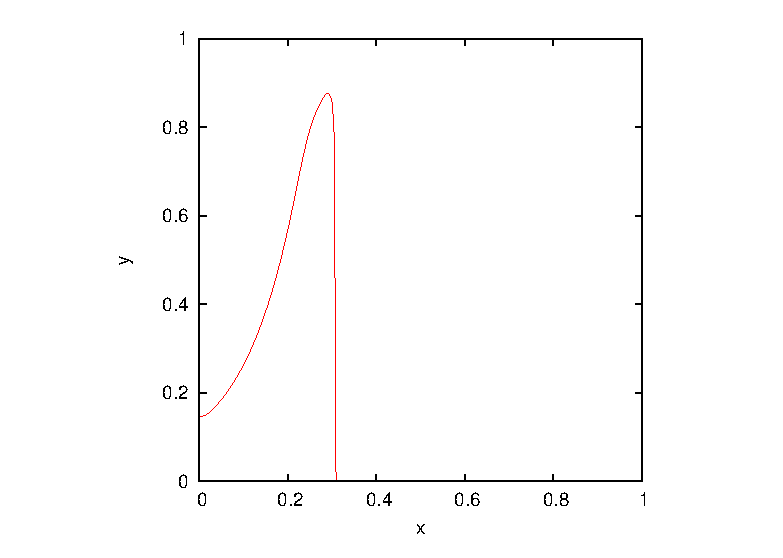
\includegraphics[scale=0.55]{trav_wave_solution_t20.eps} \\
      (a) & (b) \\
      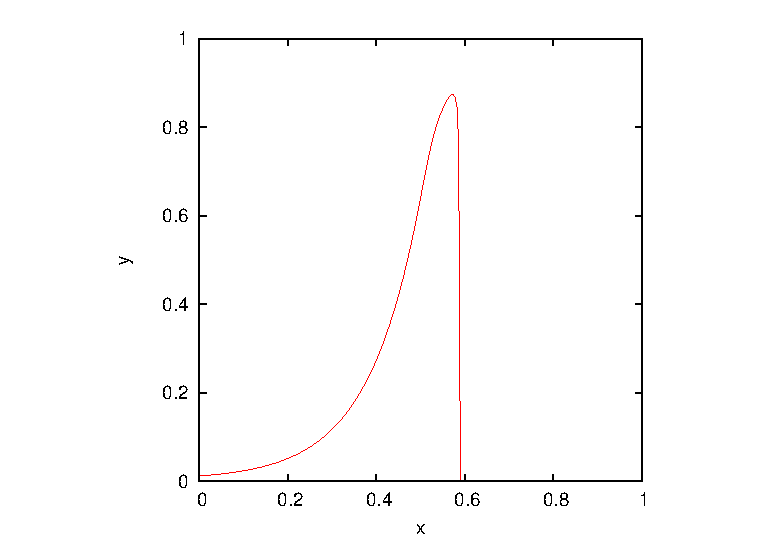
\includegraphics[scale=0.55]{trav_wave_solution_t40.eps} & 
      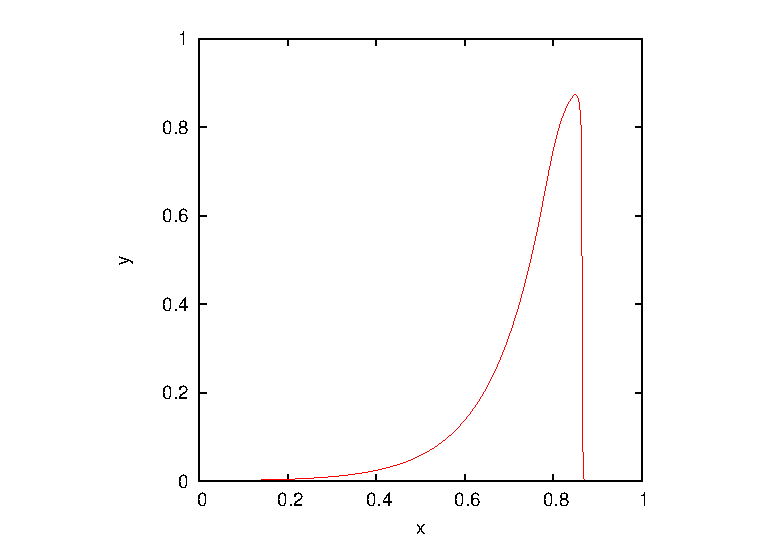
\includegraphics[scale=0.55]{trav_wave_solution_t60.eps} \\
      (c) & (d) 
  \end{tabular}
  \caption{Solutions of $M(x,t)$ and $C(x,t)$ at (a) t = 0, (b) t = 20, (c) = 40, (d) = 60. 
    This was run on a $513 \times 4$ grid.}
  \label{fig:trav_wave_solution}
\end{figure}

The existence of a travelling wave solution for this simulation can be confirmed if the solution $M(x,t)$ can be shown as $M(x-ct)$, where $c$ is the \textit{a priori} unknown wave speed.
This can be graphically confirmed by horizontally translating the solution at different time steps on top of each other.
If the superimposed solutions are of similar shape and have been translated by multiples of the same value then evidence of a travelling wave would be shown.
This would suggest that the value used for horizontal translations is an approximation for the wavespeed $c$. 
We can numerically approximate the value for $c$ by looking at how fast the peak of the wave travels.
The location of the wave peak is the x coordinate that corresponds to the largest $M$ value.
Recall that we are dealing with a pseudo-one dimensional problem, so there does not need to be any consideration for an $(x,y)$ coordinate.
For this case, we used the GNUPLOT software to fit a linear model, $f(x) = mx + b$, to the last half of the wave peaks path, seen in Figure \ref{fig:trav_waveSpeed}.
The last half of the values were used instead of the whole set of values because only for the former do we have a fully formed travelling wave.
The value of $m$ in $f(x)$ is the approximation for the wave speed, $c$. 

\begin{figure}[!htp]
  \centering
    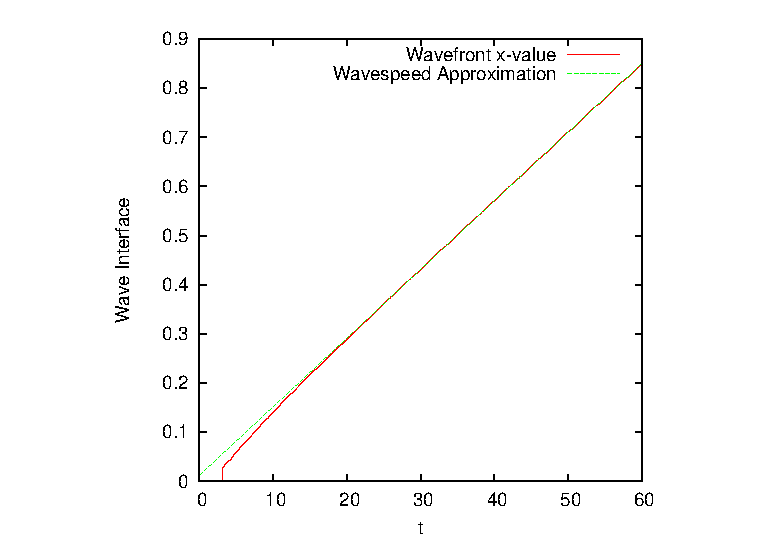
\includegraphics[scale=0.85]{trav_wavespeed.eps}
    %!% At some point, try to get a line in the graphic that show the region that was used for the fitting.
    \caption{The $x$ location of the wave peak as a function of $t$.
      The red line is the wave peak location extracted from the simulation results.
      The green line is the function $f(x) = cx + b$ with c as the wave speed, found by fitting the model to the second half of x values.
      The simulation results used here are from the solution shown in the previous Figure.
    }
    \label{fig:trav_waveSpeed} 
\end{figure}

With an approximation for $c$, the solutions of Figure \ref{fig:trav_wave_solution} can be represented as $M(x - c (t_0 - t_{n}))$, where $t_0 = 60$ is a reference point for the other time steps.
The values of $t_{n}$ are the times for the other solutions.
By translating along the $x$-axis multiple solution profiles can be superimposed, as seen in Figure \ref{fig:trav_wave_translation}.
The shape of each time step is very similar throughout, only differing slightly at the tail.

\begin{figure}[!htp]
  \centering
    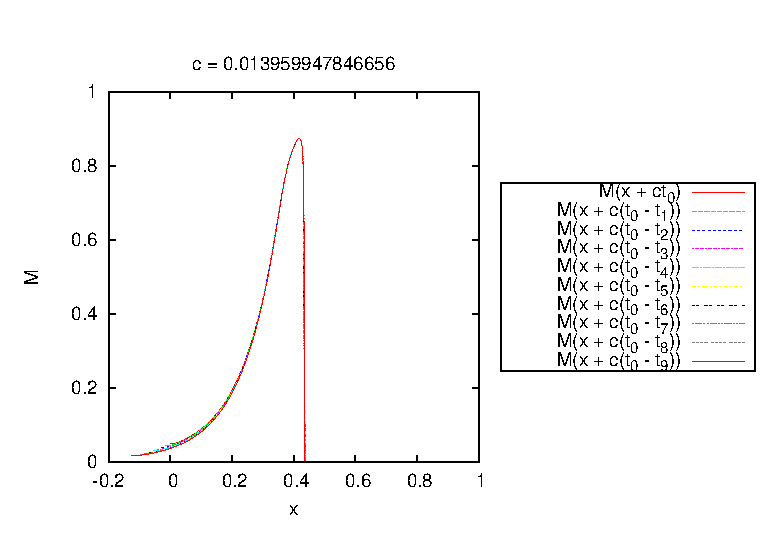
\includegraphics[scale=0.85]{trav_wave_translation.eps}
    \caption{Solutions of $M$ that are represented as $M(x -ct)$ \textit{a priori}.
      The multiple time steps are translated on top of another by horizontal movements of $c (t_0 - t_n)$ for each time step.
      }
    \label{fig:trav_wave_translation}
\end{figure}

Based on the above evidence, we can say that a travelling wave solution has been suggested to exist numerically for a single initial condition and particular set of parameters.
This leads to two logical extensions, looking at the stability of the travelling wave solution based on initial condition and investigating the effect the parameters have on the travelling wave solution.

%%%%%%%%%%%%%%%%%%%%%%%%%%%%%%%%%%%%%%%%%%%%%%%%%%%%%%%%%%%
\subsection{Travelling Wave Stability}

%!% section 4.2.3 not sure that the important thing is really that the wave becomes a 1D solution  ... we can discuss tomorrow or in your exam.
%!% section 1.2.3:  it seems that you are here interested in whether you obtain a 1D travelling wave, i.e. you measure whether your solution deviates from a 1D solution. I am not certain that this is the relevant question. I think the question is whether in a full 2D case you get a travelling wave (which does not need to be a 1D wave but can be a fully 2D solution). Your figure \ref{trav_wavefront} seems to suggest this. We can talk about this in the exam or next week.

Based on the previous example, there seems to exist a travelling wave solution for the intial condition given in (\ref{equ:basic_init_trav_wave}).
The next step is looking at how different initial conditions could still result in a travelling wave solution.
For this we specifically look at the stability of the solution, does it attract each nearby solution into becoming a travelling wave solution or do only special cases become travelling wave solutions.
This will help confirm that the existence of the travelling wave solution is not dependent on the single choice of initial condition.

To test this we take an initial condition that is not inherently one dimensional and see if it approaches the one dimensional property.
The choice of IC is to have multiple random spherical inoculation points along the $y=0$ side of the region.
Specifically, we use $(x_r, y_r)$ to represent the center of each random inoculation point.
Here $x_r \in \mathcal{R}$ and $y_r \in [0, 0.1]$.

The equation used for each random spherical inoculation point is,
\begin{equation}
  M = \frac{-h}{d^2} \left( (x - x_r)^2 + (y - y_r)^2 \right) + h, \quad M \ge  0.
\end{equation}
Random inoculation points add to each other if they overlap.
After all the inoculation points have been generated, every value is divide by the total amount of biomass.
This lets the initial condition become a representation for the distribution of random inoculation points in terms of the total amount generated.
A time evolution of the simulation with the above initial condition can been seen in Figure \ref{fig:trav_stability}.
Here it can be observed that the solution $M$ appears to slowly converge to a one dimensional problem.
This cannot be fully seen since the wave propagation reaches the end of the region before it can become fully one dimensional.

\begin{figure}[!htp]
  \centering
  \begin{tabular}{c c}
      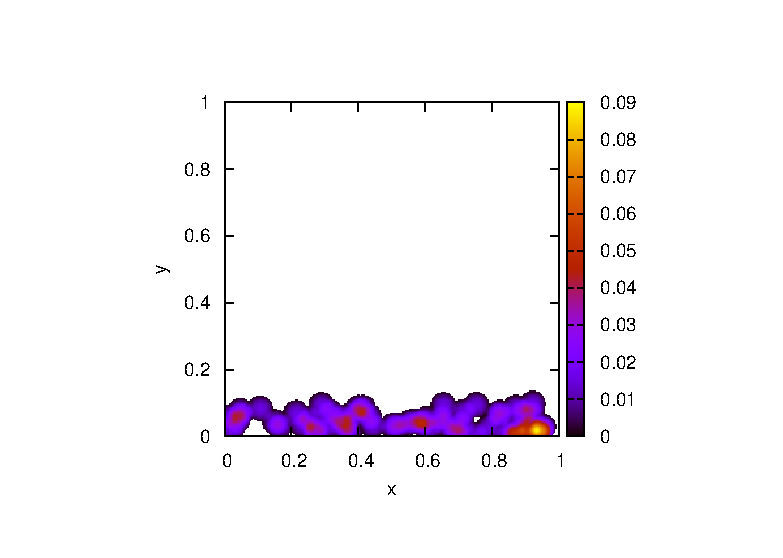
\includegraphics[scale=0.52]{trav_stability_t0.eps} &
      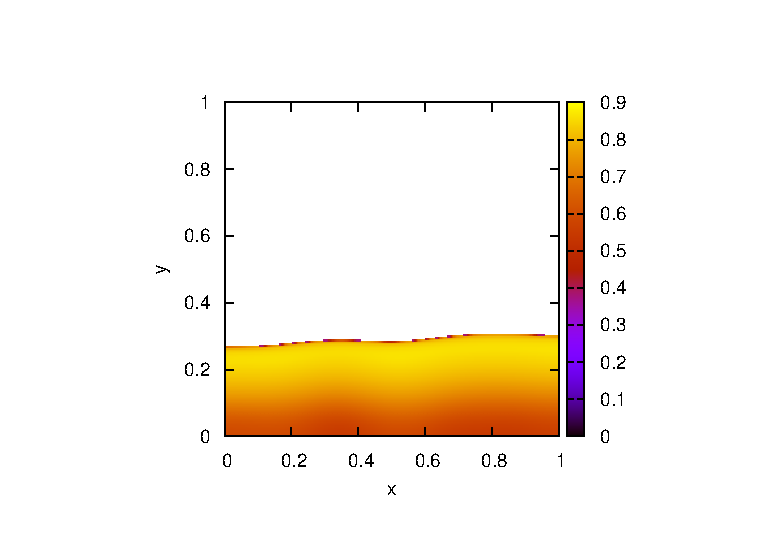
\includegraphics[scale=0.52]{trav_stability_t10.eps} \\
      (a) & (b) \\
      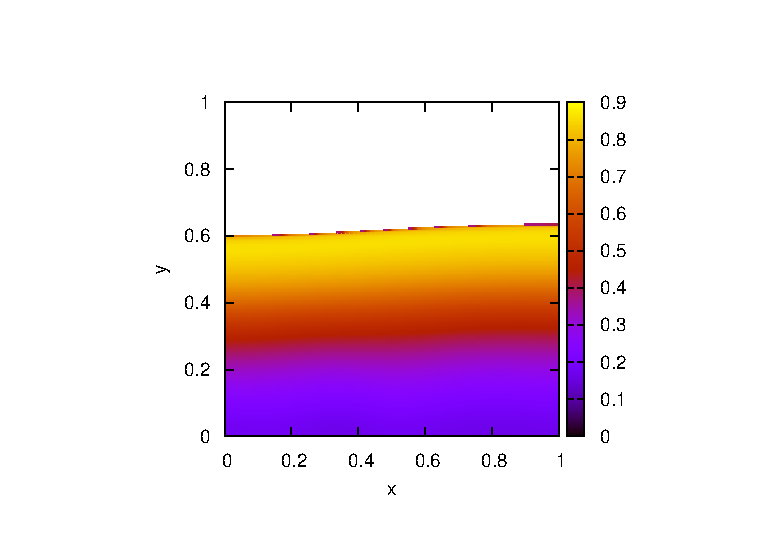
\includegraphics[scale=0.52]{trav_stability_t20.eps} &
      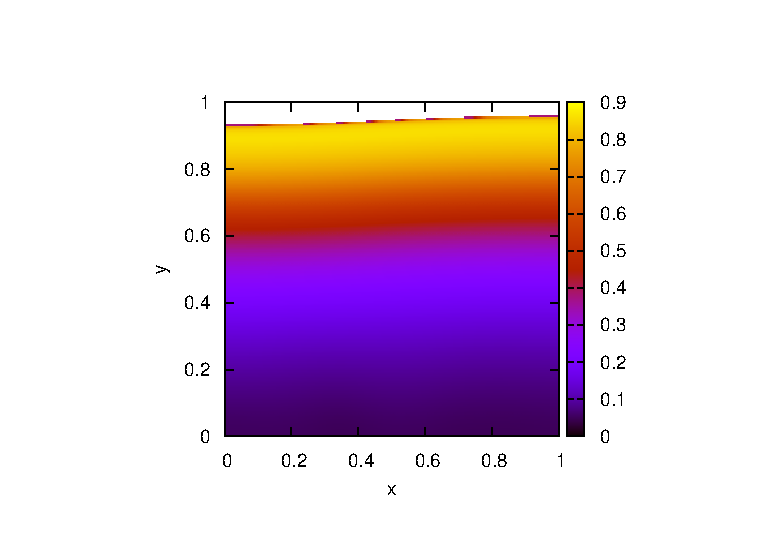
\includegraphics[scale=0.52]{trav_stability_t30.eps} \\
      (c) & (d) 
  \end{tabular}
  \caption{Plots of the simulation with random spherical inoculation points centered in the region $(x,y) \in [0,0] \times [1,0.1]$.
    The solutions are shown at (a) $t = 0$, (b) $t = 10$, (c) $t = 20$, and (d) $t = 30$.
    Each solution is computed on a $513 \times 513$ grid. }
  \label{fig:trav_stability}
\end{figure}

\begin{figure}[!htp]
  \centering
  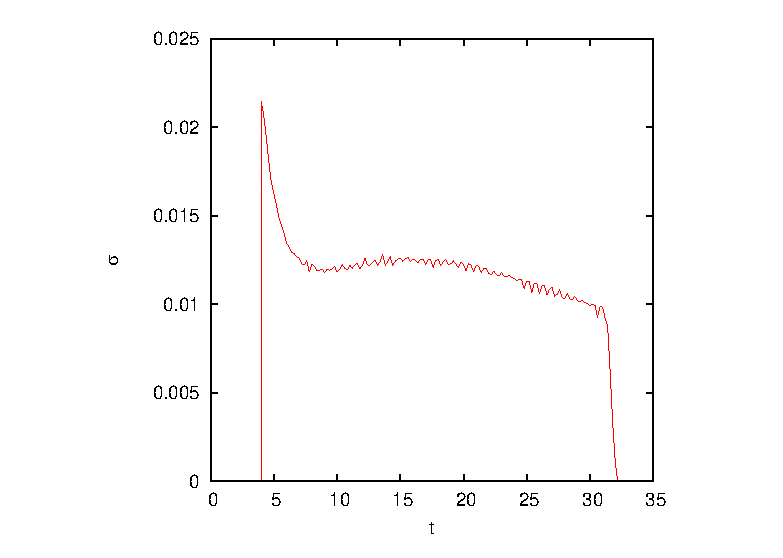
\includegraphics[scale=0.95]{trav_stability.eps}
  \caption{The standard deviation of the wavefront interface as a function of time.
    The wavefront references the largest $y$ coordinate with $M > 0.001$ for each $x$ coordinate.
    The choice of using $M > 0.001$ is because we want to ignore the small values ($~10^{-100}$) that arise from the diffusion right at the wave front. 
    This simulation is the same as the previous Figure.  }
  \label{fig:trav_stability_stddev}
\end{figure}

We can quantitatively see the behaviour of this convergence by calculating the measure of spread at the wave front.
This can be achieved by calculating the standard deviation of $y$ coordinated for each x coordinate.
By tracking the largest $y$ value with a non-zero $M$ for each $x$ value we can generate a sample data set of the wavefront.
The wavefront is used instead of other points of interest, such as the wave peak, because it is the most consistent of characteristics that can be easily tracked.
As seen in Figure \ref{fig:show_dimension_stddev}, the wave peak had the largest spread among all other values. 

\begin{figure}[!htp]
  \centering
  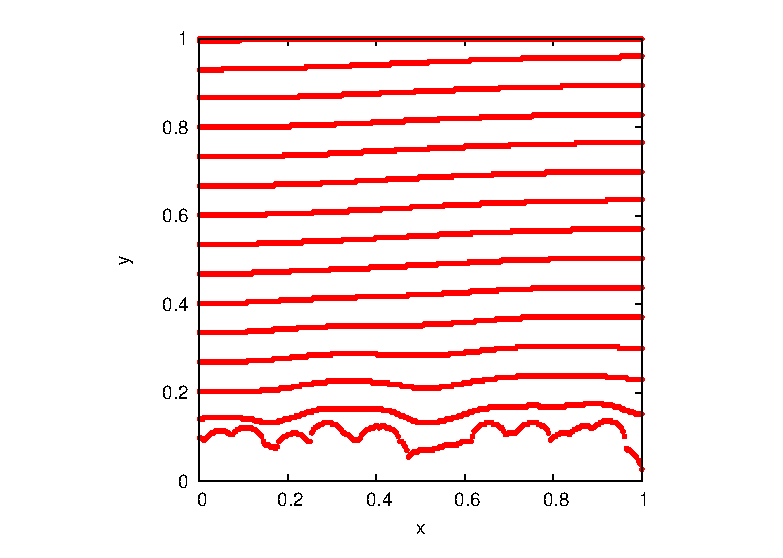
\includegraphics{trav_stability_wavefront.eps}
  \caption{The wavefront shape of multiple time steps.
    Each wavefront has a difference in time by 2, i.e. they are at $t = 4, 6, 8, \ldots, 58, 60$. 
    The simulation results are the same as the previous Figures, using the default parameter values with a grid size $513 \times 513$.
    }
  \label{fig:trav_wavefront}
\end{figure}

Taking the sample standard deviation of this set results in the measure of spread for the wavefront.
The sample standard deviation was used since this one example does not represent the whole population of solutions.
The idea is that, for a solution that converges to one-dimensionality, the $y$ location of the wavefront should be converging to similar values.
This means that the standard deviation would converge to zero.
The standard deviation of the wavefront as a function of time of the simulation ran in Figure \ref{fig:trav_stability} can be seen in Figure \ref{fig:trav_stability_stddev}.
Here is shown that the solution is converging to zero, however not monotonically.
%!% I'm actually not sure what this means.... good news or bad?!

For the numerical computation of the wavefront, the largest $y$ values greater then $0.001$ was used instead of $0$.
The reason is that there are very small values of around $10^{-200}$ that arise due to the diffusion that were not adequate representations of the wavefront.

Another interesting item to investigate is the actual shape of the wavefront.
Figure \ref{fig:trav_wavefront} shows only the wavefront shape for multiple time steps.
The wavefront shape is the same dataset of points used to calculate the standard deviation of the wavefront interface.
Of interest is that the wavefront seems to move at a constant speed, since each wavefront shown is equidistance from the next.


%!% Maybe need to try other types of initial conditions to say this for sure...
% Or maybe just run this same experiment 5 or so times to get a better sample and then just show the stddev of all 5 on a single graph. If they all converge to 0ish then that looks pretty strong.


%%%%%%%%%%%%%%%%%%%%%%%%%%%%%%%%%%%%%%%%%%%%%%%%%%%%%%%%%%%
%!% Here I kinda want to show how the wavespeed dectector script works versus when I use the gnuplot fitting to calculate the wavespeed approximation.
% So here a mention the difference between each calculation and then show the horizontal translation graph for both the script and the fitted wavespeed.
%Show computations for the wave speed

%%%%%%%%%%%%%%%%%%%%%%%%%%%%%%%%%%%%%%%%%%%%%%%%%%%%%%%%%%%
\subsection{Parameter Effect on Wave Speed}

The travelling wave solutions seen before have all existed for a single set of parameters.
Here the four main system parameters, $\delta$, $\kappa$, $\nu$, and $\gamma$ are independently varied and the effect on the travelling wave solutions are observed.
From this we can also see how the wave speed of the travelling wave solution changes as a function of the different model parameters.

\begin{figure}[!htp]
  \centering
  \begin{tabular}{c c}
    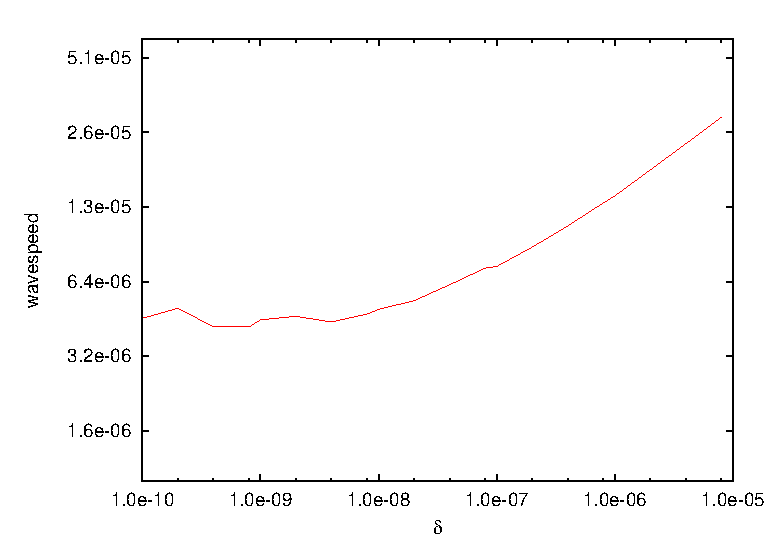
\includegraphics[scale=0.55]{parameter_speed_delta.eps} &
    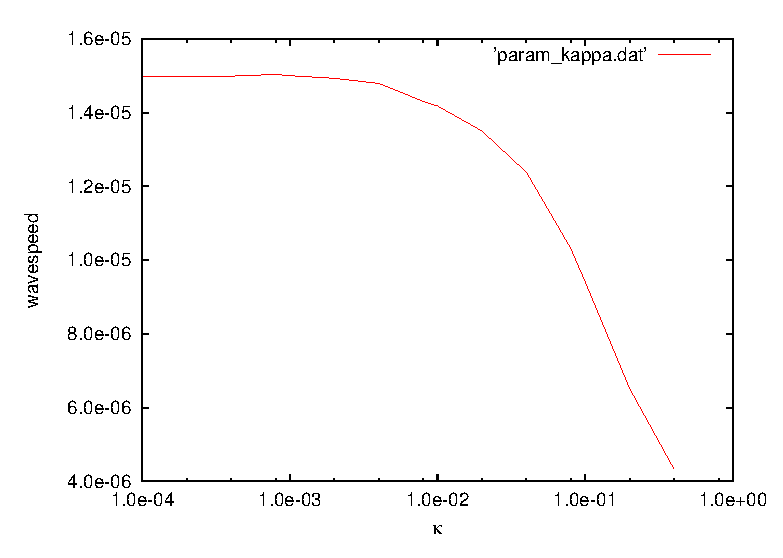
\includegraphics[scale=0.55]{parameter_speed_kappa.eps} \\
    (a) & (b) \\
    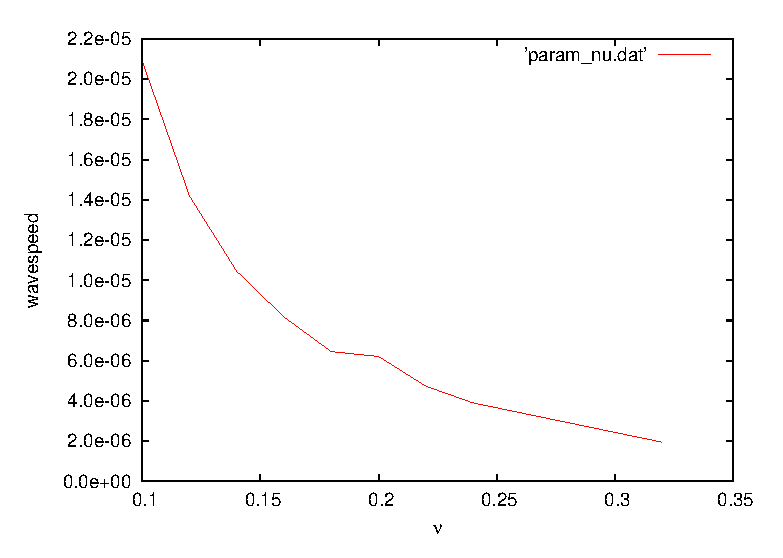
\includegraphics[scale=0.55]{parameter_speed_nu.eps} &
    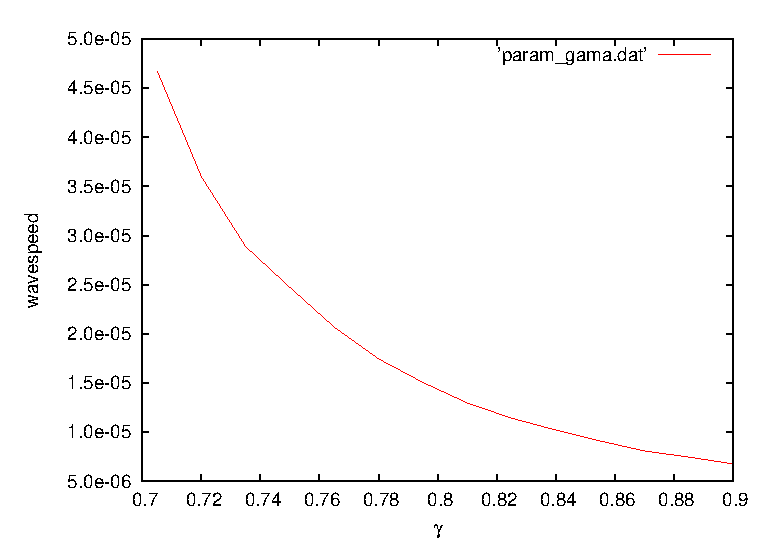
\includegraphics[scale=0.55]{parameter_speed_gama.eps} \\
    (c) & (d) 
  \end{tabular}
  %!% Figure 1.14. the fonts i think are too small; these changes can be made later, not crucial for approving the thesis for defense
  \caption{The value of $c$ as parameter (a) $\delta$, (b) $\kappa$, (c) $\nu$, and (d) $\gamma$ are changed. 
    Note that (a) and (b) have logscales due to the selection of parameter values.
    Each of these were calculated with the same setup as the travelling solution previously done.
    The grid size for each was $513 \times 4$ and a time step of $\Delta t = 0.001$ was used.}
  \label{fig:parameter_speed}
\end{figure}

For this an automated script was created that checks, for each time step, if $M$ is travelling wave solution based on the solution $M$ from a number of time steps previous.
From this check, a wave speed needs to be approximated based on the distance between the two solutions.
If this approximated wave speed is matched throughout all the x values, then a travelling wave solution is assumed to exist at that time step.
With this script, we can try the same simulation as Figure \ref{fig:trav_wave_solution} with different parameter values.

For each parameter, $\delta$, $\kappa$, $\nu$, $\gamma$, the range of values chosen were arbitrarily.
Figure \ref{fig:parameter_speed} shows the results of the wave speed for each parameter changes.
Mainly it was so that the solution did not propagate too fast and hit the end of the region before developing into a full travelling wave solution.
Generally when the travelling wave does not form it is because the wave front propagates to the end of the region faster then the tail of the travelling wave can decrease to 0.
In the case of $\nu$, any larger values than the selected range resulted in biomass that died faster then it could grow, and thus no travelling wave solution exists.
There did not appear to be any cases were a travelling wave solution could not form.

The behaviour of the wave speed as a result of changing the parameters can be explained by the biological meaning of each parameter.
For $\delta$, the diffusion constant, a large value results in a larger local biomass growth as a result of diffusion.
This speeds up the spreading of the biomass and the propagation of the interface.
For $\kappa$, the half-saturation concentration, this value depicts at what substrate concentration we achieve half-maximum growth for the biomass.
When this value is large, the required amount of substrate for optimal growth speed is increased and thus the overall growth of the biofilm is slowed down.
For $\nu$, the decay and loss rate of biomass, a larger value results in more biomass being ejected from the system and thus the amount of biomass available to grow become smaller and growth propagations are slowed.
For $\gamma$, the biomass yield coefficient, a larger value correlates to a substrate that is quickly consumed which produces less total biomass for growth.
This inhibits the propagation of the biomass interface and lowers the wave speed.
The simulated values recorded in Figure \ref{fig:parameter_speed} agree with the expected behaviour for each parameter.



